\chapter{Σχεδιασμός εφαρμογής}
\label{chap3}
\begin{figure}[!htb]
	%\vspace{2px}%
	\centering
	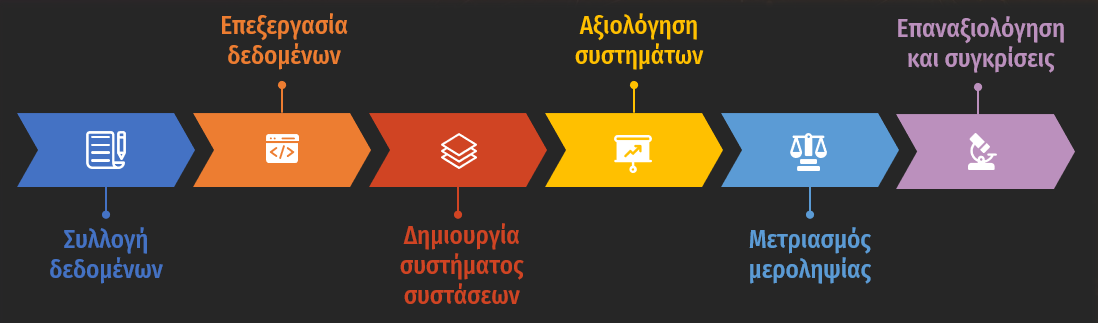
\includegraphics[width=\linewidth]{experiment.png}
	\caption{Δομή πειράματος}
	\label{fig:exp}
\end{figure}
\noindent Το πείραμα που υλοποιήθηκε στα πλαίσια αυτής της εργασίας αποτελείται από 6 βασικά στάδια, όπως φαίνεται και στην Εικόνα \ref{fig:exp}. Στο πρώτο στάδιο γίνεται η εύρεση και η συλλογή των πιο κατάλληλων συνόλων δεδομένων για τη συγκεκριμένη εργασία. Ακολουθεί η κατάλληλη επεξεργασία και οπτικοποίηση των δεδομένων που επιλέχθηκαν, κάτι που είναι απαραίτητο για την καλύτερη κατανόηση των δεδομένων μας και την προετοιμασία τους για να δοθούν ως είσοδος στους αλγορίθμους συστάσεων. Έπειτα, επιλέγονται οι αλγόριθμοι συστάσεων που θα παράξουν τις αρχικές λίστες συστάσεων για τους χρήστες και φυσικά οι πιο κατάλληλες τιμές των υπερπαραμέτρων τους. Αφού παραχθούν οι λίστες, ακολουθεί η αξιολόγηση των αλγορίθμων ως προς την ακρίβεια, το popularity bias, το diversity, το coverage και το novelty. Με τον όρο coverage, αναφερόμαστε στα συνολικά αντικείμενα που καλύπτει ο αλγόριθμος κατά την παραγωγή συστάσεων από τα διαθέσιμα αντικείμενα. Επόμενο στάδιο αποτελεί η χρήση τεχνικών για την μετριασμό της μεροληψίας που (ενδεχομένως) εντοπίστηκε στο προηγούμενο βήμα και η παραγωγή νέων λιστών συστάσεων. Τέλος, γίνεται η αξιολόγηση των νέων αποτελεσμάτων και σύγκριση με τα αρχικά αποτελέσματα που είχαν προκύψει ύστερα από τη δημιουργία των αρχικών λιστών συστάσεων.\\\\
Για την εκτέλεση όλων των βημάτων του πειράματος, κρίθηκε απαραίτητη η δημιουργία μιας διαδικτυακής εφαρμογής (web-app), η οποία έλαβε το όνομα \textit{``Bias \& Fairness in RecSys"}. Μια διαδικτυακή εφαρμογή είναι μια εφαρμογή η οποία είναι προσβάσιμη μέσω του διαδικτύου, χρησιμοποιώντας έναν οποιοδήποτε φυλλομετρητή (browser). Η επιλογή μιας διαδικτυακής εφαρμογής προκρίθηκε έναντι μιας εφαρμογής για υπολογιστή ή κινητό, καθώς είναι ανεξάρτητη από το λειτουργικό σύστημα που έχει το σύστημα του χρήστη. Έτσι αφενός μεν δεν χρειάζεται να δημιουργηθούν διαφορετικές εκδόσεις ανάλογα με το λειτουργικό σύστημα και αφετέρου δε είναι αρκετά πιο εύκολη η πρόσβαση για έναν χρήστη, διότι δεν χρειάζεται να εγκαταστήσει κάποιο πρόγραμμα στο σύστημά του.\\\\
\noindent Η υλοποίηση της διαδικτυακής εφαρμογής (web-app) έγινε στη γλώσσα προγραμματισμού Python (έκδοση 3.8.7) με χρήση του ανοιχτού κώδικα framework Streamlit \cite{StreamlitFastestWay} (έκδοση 1.0.0), το οποίο χρησιμοποιείται ευρέως για τη δημιουργία web-apps για εργασίες μηχανικής μάθησης, επιστήμης των δεδομένων και βαθιάς μάθησης. Το κύριο πλεονέκτημα του Streamlit είναι πως δεν απαιτείται η γνώση front-end τεχνικών, όπως HTML, CSS, JavaScript για τη δημιουργία μιας εφαρμογής και είναι εφικτή η μετατροπή των κωδικών που έχουμε σε γλώσσα Python σε μια καλαίσθητη και φιλική προς τους χρήστες εφαρμογή μέσα λίγα και απλά βήματα. Η γλώσσα προγραμματισμού Python επιλέχθηκε καθώς είναι αρκετά δημοφιλής τόσο για εφαρμογές μηχανικής μάθησης, όσο και για συστήματα συστάσεων και διαθέτει μια πληθώρα βιβλιοθηκών και frameworks. Για τη συγγραφή, την εκτέλεση και την αποσφαλμάτωση του κώδικα, επιλέχθηκε το PyCharm IDE (Integrated Development Environment - ολοκληρωμένο περιβάλλον ανάπτυξης).
Οι πιο σημαντικές βιβλιοθήκες που χρησιμοποιήθηκαν είναι:
\begin{itemize}
	\item \textbf{Scikit-learn (Sklearn):} μια από τις πιο πλούσιες, χρήσιμες και απαραίτητες βιβλιοθήκες για μηχανική μάθηση. Προσφέρει μεταξύ άλλων αρκετούς αλγορίθμους μηχανικής μάθησης, αρκετά χρήσιμα εργαλεία και ορισμένα σύνολα δεδομένων.
	\item \textbf{Pandas:} βιβλιοθήκη για τη διαχείριση και την ανάλυση δεδομένων. Προσφέρει δομές δεδομένων και εργαλεία για προβολή και διαχείριση χρονοσειρών.
	\item \textbf{Altair:} βιβλιοθήκη για τη δημιουργία διαδραστικών γραφημάτων.
	\item \textbf{NumPy (Numerical Python):} πρόκειται για την βασική βιβλιοθήκη επιστημονικού υπολογισμού στην Python, προσφέρει διάφορα εργαλεία για την αποδοτική και αποτελεσματική διαχείριση μητρώων και εκτέλεση διάφορων πράξεων επ'αυτών.
	\item \textbf{Plotly:} βιβλιοθήκη για τη δημιουργία διαδραστικών γραφημάτων.
\end{itemize}
\begin{table}[H]
	\centering	
	\caption {Σύγκριση frameworks} \label{tab:framework}
	\begin{tabular}{|l|l|l|l|ll|}
		\hline
		& Αλγόριθμοι & \shortstack{Αλγόριθμοι για \\ μετριασμό μεροληψίας} \rule{0mm}{9mm} & \shortstack{Μετρικές \\ (σύνολο)} & \shortstack{Μετρικές \\ C.N.D.B.F. \footnotemark{} } &  \\ \hline
		DaisyRec    & 19         &       0     & 10       & 0        &  \\ \hline
		Elliot     & 50         &        0    &       36   &      22    &  \\ \hline
		Lenskit            &       6     &      0     &       6     &      0    &  \\ \hline
		Librec-auto &   55         &       7      &     10     &   14       &  \\ \hline
		Surprise   &       7     & 0          &      4    & 0        & \\ \hline
	\end{tabular}
\end{table}
\footnotetext{C.N.D.B.F.: CoverageNoveltyDiversityBiasFairness}
Με αυτόν τον τρόπο το “Bias \& Fairness in Recsys” αποτελεί όχι μόνο ένα εργαλείο ανάλυσης και μετριασμού της μεροληψίας, αλλά και μια εφαρμογή μέσω της οποίας μπορούν να αναπτυχθούν συστήματα συστάσεων με εύκολο και αρκετά φιλικό προς τον χρήστη τρόπο.
Για την επιλογή του framework (εργαλείου)  που θα μας δώσει τους αλγορίθμους για να δημιουργήσουμε τα συστήματα συστάσεων έγινε σύγκριση των frameworks:  Surprise \cite{hugSurprisePythonLibrary2020}, librec-auto \cite{mansouryAutomatingRecommenderSystems2018}, Elliot \cite{anelliElliotComprehensiveRigorous2021}, DaisyRec \cite{sunAreWeEvaluating2020}, Lenskit \cite{ekstrandLensKitPythonNextGeneration2020}. Τα βασικά κριτήρια για την τελική επιλογή ήταν το πλήθος των αλγορίθμων και των μετρικών που προσέφεραν, η επεκτασιμότητα και η ύπαρξη όσο το δυνατόν πιο καλογραμμένων και πληρέστερων εγγράφων τεκμηρίωσης (documentation). Με βάση αυτά έγινε η ανάλυση που βλέπουμε στον Πίνακα \ref{tab:framework} και επιλέχθηκε το Elliot framework για τη δημιουργία των αρχικών προτάσεων από τους base αλγορίθμους συστημάτων συστάσεων.

%\begin{lstlisting}[caption={Παράδειγμα yaml αρχείου στο Elliot},label={lst:yml},style=mystyle]
\begin{lstlisting}[caption={Παράδειγμα yaml αρχείου στο Elliot},label={lst:yml},style=mystyle]
experiment:
	dataset: movielens_1m
	data_config:
		strategy: fixed
		train_path: data/movielens_1m/splitting/train.tsv
		test_path: data/movielens_1m/splitting/test.tsv
	path_output_rec_result: Thesis/Results
	path_output_rec_performance: Thesis/Results
	splitting:
		save_on_disk: True
		save_folder: data/movielens_1m/splitting/
		test_splitting:
			strategy: random_subsampling
			test_ratio: 0.2
	top_k: 50
	evaluation:
		cutoffs: [50, 30, 20, 10]
		simple_metrics: [nDCG,Precision, Recall, ItemCoverage,EPC,Gini,HR,ARP,ACLT,APLT, PopREO, PopRSP]
		relevance_threshold: 0
	gpu: 1
	external_models_path: elliot-master/external/models/__init__.py
	models:
		ItemKNN:
			meta:
				verbose: True
				save_recs: True
				validation_metric: nDCG@10
			neighbors: [50, 70]
			similarity: cosine
			implementation: classical
		UserKNN:
			meta:
				verbose: True
				save_recs: True
				validation_metric: nDCG@10
			neighbors: [ 50,70 ]
			similarity: cosine
			implementation: classical
\end{lstlisting}
%\begin{figure}[!htb]
%	%\vspace{2px}%
%	\centering
%	\includegraphics[width=\linewidth]{elliot_yml.png}
%	\caption{Παράδειγμα yml αρχείου στο Elliot framework}
%	\label{fig:yml}
%\end{figure}

\noindent Στο Elliot framework είναι αρκετά απλή η εκτέλεση ενός πειράματος για διαφορετικούς αλγορίθμους και η αξιολόγηση από τις μετρικές που επιθυμούμε δημιουργώντας απλά ένα αρχείο τύπου .yaml. Ένα παράδειγμα τέτοιου αρχείου δίνεται στον κώδικα \ref{lst:yml}.
 Ακόμη υπάρχει και η δυνατότητα για ρύθμιση υπερπαραμέτρων (hyperparameter tuning) επιλέγοντας ανάμεσα σε 51 στρατηγικές. Τέλος, το Elliot δίνει την δυνατότητα για στατιστικές δοκιμές.\\
Η εφαρμογή ``Bias \& fairness in Recsys" περιέχει 7 διαφορετικές σελίδες στις οποίες μπορεί να πλοηγηθεί ο χρήστης:

\begin{enumerate}
	\item Αρχική (Home) 
	\item Οπτικοποίηση δεδομένων (Visualize data)
	\item Δημιουργία συστημάτων συστάσεων (Build recommendation systems)
	\item Αξιολόγηση αποτελεσμάτων (Bias identification)
	\item Μετριασμός μεροληψίας (Bias mitigation)
	\item Επεξήγηση μετρικών (Metrics explanation)
	\item Μεταφόρτωση δεδομένων (Upload data)
\end{enumerate}
Η εφαρμογή υποστηρίζει δύο γλώσσες ελληνικά και αγγλικά, η εναλλαγή μεταξύ των οποίων είναι αρκετά εύκολη. Θα πρέπει να σημειωθεί πως για όλα τα γραφήματα που παρουσιάζονται στους χρήστες σε κάθε σελίδα της εφαρμογής υπάρχει η δυνατότητα να τα αποθηκεύσουν στο σύστημά τους ή/και να τα επεξεργαστούν (να εστιάσουν στο σημείο που θέλουν). Ακολουθεί η αναλυτική περιγραφή όλων των σελίδων της εφαρμογής, ενώ σε όλες τις περιπτώσεις η γλώσσα της εφαρμογής που θα χρησιμοποιήσουμε θα είναι η ελληνική.
\section{Αρχική σελίδα}
\noindent Στην αρχική σελίδα παρουσιάζονται ορισμένες πληροφορίες για τη δομή του πειράματος και της εφαρμογής. Επίσης, στον χρήστη δίνονται αναλυτικές οδηγίες για τη χρήση της εφαρμογής και την υλοποίηση του πειράματος μέσω αυτής.
Ο χρήστης έχει τη δυνατότητα να πλοηγηθεί στις σελίδες ώστε να εκτελέσει τα βήματα του πειράματος με τη σειρά που αναφέρονται ή να ακολουθήσει ορισμένες μόνο φάσεις του πειράματος με οποιαδήποτε σειρά επιθυμεί ο ίδιος.
\begin{figure}[!htb]
	%\vspace{2px}%
	\centering
	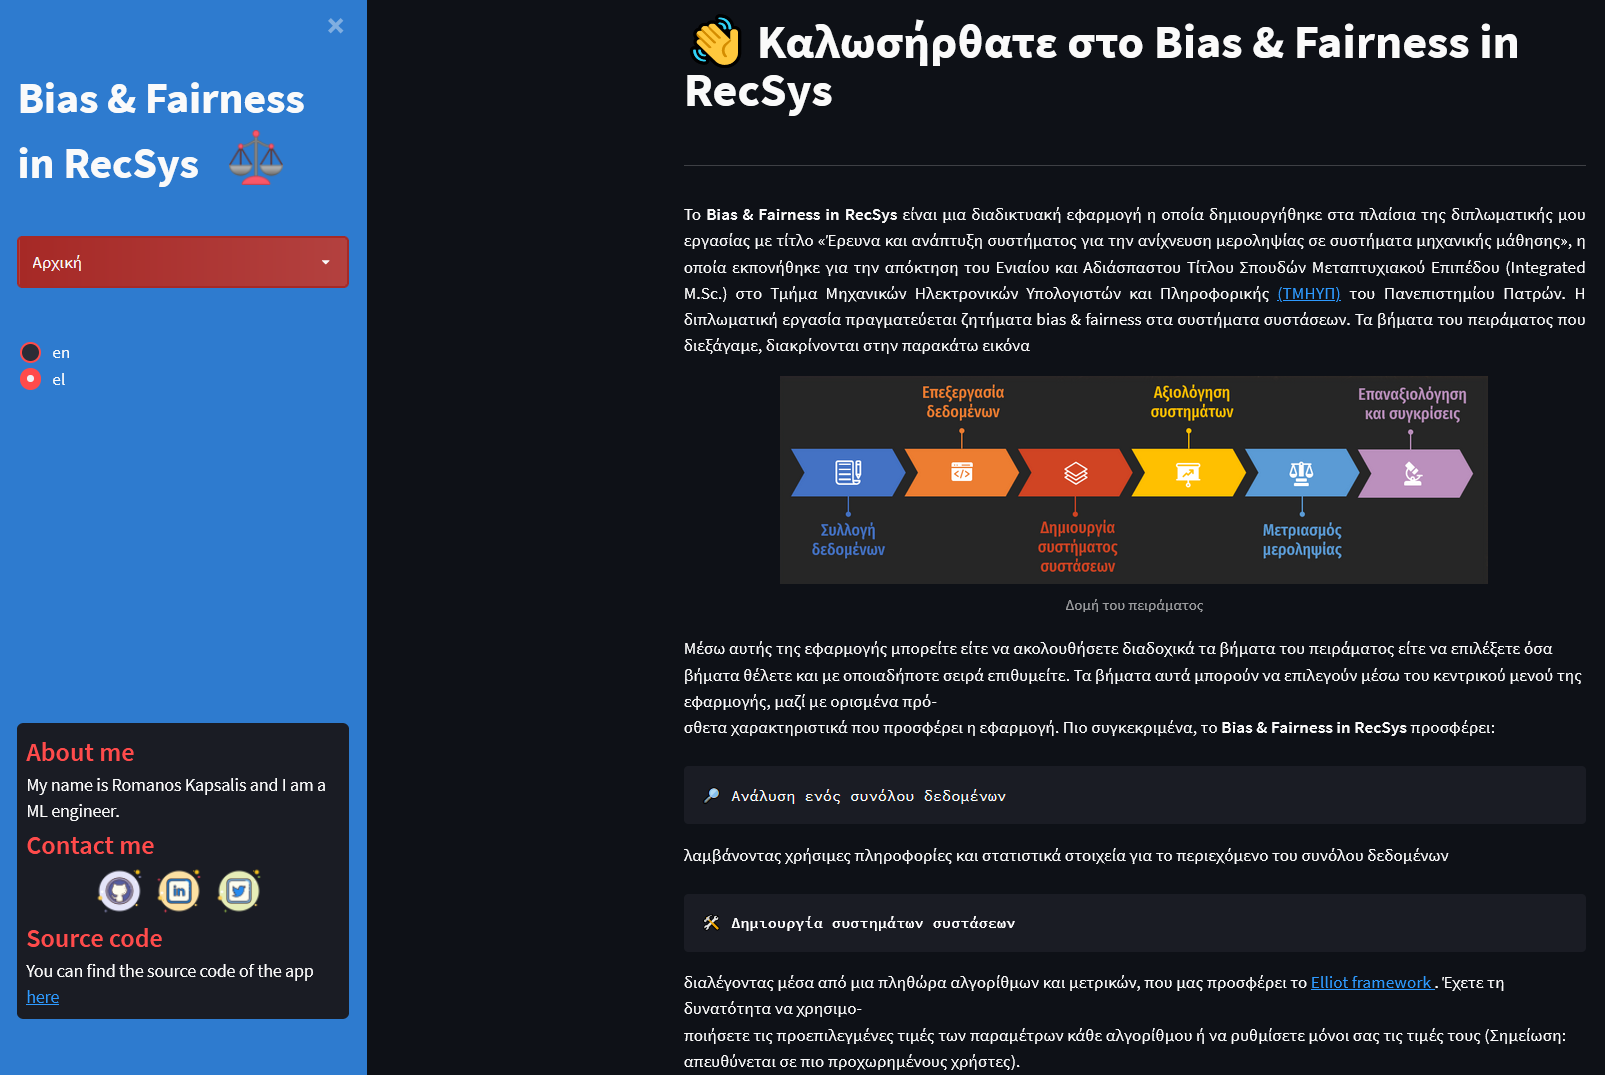
\includegraphics[width=\linewidth]{main.png}
	\caption{Αρχική σελίδα}
	\label{fig:main}
\end{figure}
\section{Οπτικοποίηση δεδομένων}
\noindent Σε αυτή τη σελίδα αρχικά επιλέγουμε ένα σύνολο δεδομένων που επιθυμούμε να αναλύσουμε και ακολούθως προβάλλονται στην οθόνη ορισμένα χρήσιμα στατιστικά στοιχεία αυτού του συνόλου δεδομένων, γραφήματα και πίνακες που το περιγράφουν. Όσον αφορά τα στατιστικά στοιχεία, για όλα τα σύνολα δεδομένων προβάλλεται ο αριθμός των χρηστών, των αντικειμένων και των αξιολογήσεων, η αραιότητα του μητρώου χρηστών-αντικειμένων, το rating space, ο λόγος των χρηστών προς τα αντικείμενα, ο λόγος των αξιολογήσεων προς τα αντικείμενα και ο λόγος των αξιολογήσεων προς τους χρήστες.\\
Τα γραφήματα δίνουν στον χρήστη χρήσιμες πληροφορίες για ένα σύνολο δεδομένων προκειμένου να κατανοήσει καλύτερα τη δομή και την κατανομή των δεδομένων που υπάρχουν σε αυτό, δηλαδή των χρηστών, των αντικειμένων και των αξιολογήσεων στην περίπτωσή μας. Το πρώτο γράφημα που προβάλλεται παρουσιάζει τα πιο δημοφιλή προϊόντα, ως προς τον αριθμό των αξιολογήσεων που έχουν λάβει, παρέχοντας μάλιστα τη δυνατότητα επιλογής του αριθμού των πιο δημοφιλών αντικειμένων που επιθυμούμε. Το επόμενο γράφημα μας δίνει τους κορυφαίους χρήστες, ως προς τον αριθμό των αξιολογήσεων που έχουν πραγματοποιήσει και εδώ όπως και στο προηγούμενο γράφημα, παρέχεται η δυνατότητα επιλογής του αριθμού των πιο δημοφιλών χρηστών που επιθυμούμε να προβάλλουμε. Ένα αρκετά χρήσιμο γράφημα, ειδικά αν θέλουμε να δημιουργήσουμε συστήματα συστάσεων, αποτελεί η κατανομή της μέσης τιμής των αξιολογήσεων για όλα τα αντικείμενα. Τέλος, θα αποτελούσε σημαντική παράλειψη αν δεν παρουσιάζαμε το γράφημα του long tail, το οποίο σχετίζεται άμεσα με το popularity bias στα συστήματα συστάσεων. Στα σύνολα δεδομένων του Movielens που είναι διαθέσιμες και κάποιες επιπλέον πληροφορίες όπως είναι τα δημογραφικά χαρακτηριστικά των χρηστών και τα είδη των ταινιών υπάρχουν επιπλέον δύο γραφήματα, ένα για την κατανομή των ηλικιακών ομάδων των χρηστών και ένα που σχετίζεται με το φύλο και δείχνει το ποσοστό των ανδρών και των γυναικών.
\newpage
\section{Δημιουργία συστημάτων συστάσεων}
\noindent Η σελίδα «Δημιουργία συστημάτων συστάσεων» υλοποιεί ουσιαστικά το 3ο βήμα του πειράματος (Εικόνα \ref{fig:exp}), το οποίο είναι η δημιουργία των συστημάτων συστάσεων.
Η εφαρμογή προκειμένου να δημιουργήσει τα συστήματα συστάσεων συνδέεται με το Elliot framework.\\
\begin{figure}[H]
	%\vspace{2px}%
	\centering
	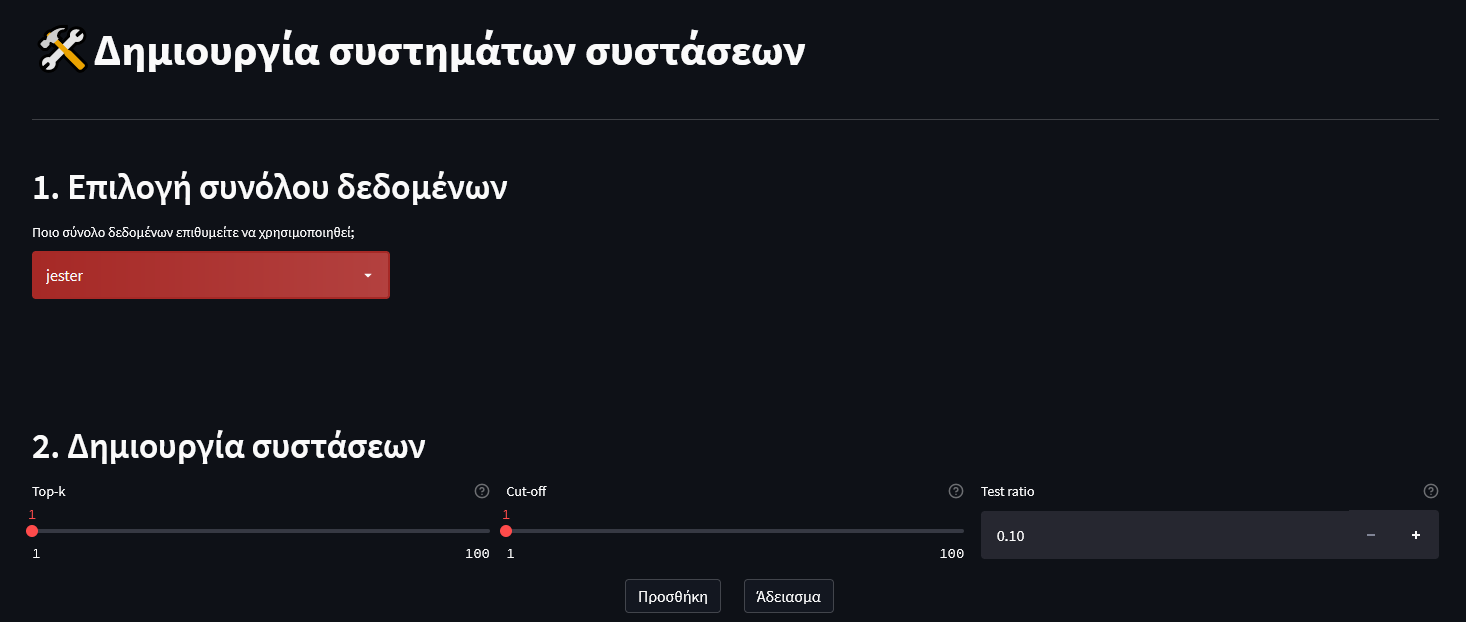
\includegraphics[width=\linewidth]{build3.png}
	\caption{Σελίδα δημιουργίας συστήματος συστάσεων}
	\label{fig:build}
\end{figure}
\noindent Πρώτα, όπως φαίνεται και στην Εικόνα \ref{fig:build} θα πρέπει να γίνει η επιλογή του συνόλου δεδομένων στο οποίο θα δημιουργηθούν τα συστήματα συστάσεων. Ο χρήστης μπορεί να επιλέξει ένα από τα σύνολα δεδομένων που χρησιμοποιήσαμε στο πείραμα ή κάποιο σύνολο δεδομένων που έχει ανεβάσει μέσω της σχετικής σελίδας («Μεταφόρτωση δεδομένων») που υπάρχει στην εφαρμογή μας. Επόμενο βήμα, είναι ο καθορισμός του μεγέθους των λιστών συστάσεων που θα δημιουργήσουν οι αλγόριθμοι (top-k), του μεγέθους ή των μεγεθών των λιστών συστάσεων που θα λάβει υπόψη της μια μετρική αξιολόγησης (cut-off) και του ποσοστού του συνόλου δεδομένων που θα χρησιμοποιηθεί για τη δημιουργία του συνόλου δοκιμής, κατά τη διάσπασή του σε δύο υποσύνολα, το σύνολο εκπαίδευσης και το σύνολο δοκιμής. Για τη χρήση παραπάνω από μίας τιμής cut-off, αφού επιλεγεί η τιμή προστίθεται στη λίστα των cut-off με το πάτημα του κουμπιού «Προσθήκη». Προφανώς όπως γίνεται αντιληπτό, θα πρέπει να ισχύει ότι cut-off  $\leq$ top-k , σε διαφορετική περίπτωση ο χρήστης λαμβάνει προειδοποιητικό μήνυμα και καλείται να αλλάξει τις τιμές ώστε να ικανοποιείται αυτός ο περιορισμός. Επίσης, με το πάτημα του κουμπιού «Άδειασμα», διαγράφονται όλες οι τιμές που εμπεριέχονται στην λίστα των cut-off, καλύπτοντας με αυτόν τον τρόπο την περίπτωση εισαγωγής λάθος τιμής από τον χρήστη. Θα πρέπει να επισημάνουμε εδώ, πως στην περίπτωση εισαγωγής μιας τιμής στην λίστα των cut-off παρουσιάζεται μήνυμα στην οθόνη το οποίο μας ενημερώνει για την επιτυχή προσθήκη μιας τιμής και για το περιεχόμενο της λίστας cut-off. Αντίστοιχο μήνυμα προβάλλεται και κατά το άδειασμα της λίστας.\\
Ακολούθως, ο χρήστης καλείται να επιλέξει τους αλγορίθμους που επιθυμεί να χρησιμοποιηθούν στο πείραμα για τη δημιουργία των συστάσεων. Οι αλγόριθμοι είναι κατηγοριοποιημένοι ανά οικογένεια αλγορίθμων, όπως φαίνεται και στην Εικόνα \ref{fig:build2}, προς διευκόλυνση των χρηστών. Σε αυτό το σημείο θα πρέπει να επισημανθεί πως δεν έχουν χρησιμοποιηθεί όλες οι οικογένειες αλγορίθμων που υπάρχουν στο Elliot, παρά μόνο όσες χρησιμοποιήσαμε στο πείραμά μας και όσες ήταν σχετικές με αυτό. Οι οικογένειες αυτές είναι: latent factor models, artificial neural networks, unpersonalized, graph based και neighborhood based.
\begin{figure}[!htb]
	%\vspace{2px}%
	\centering
	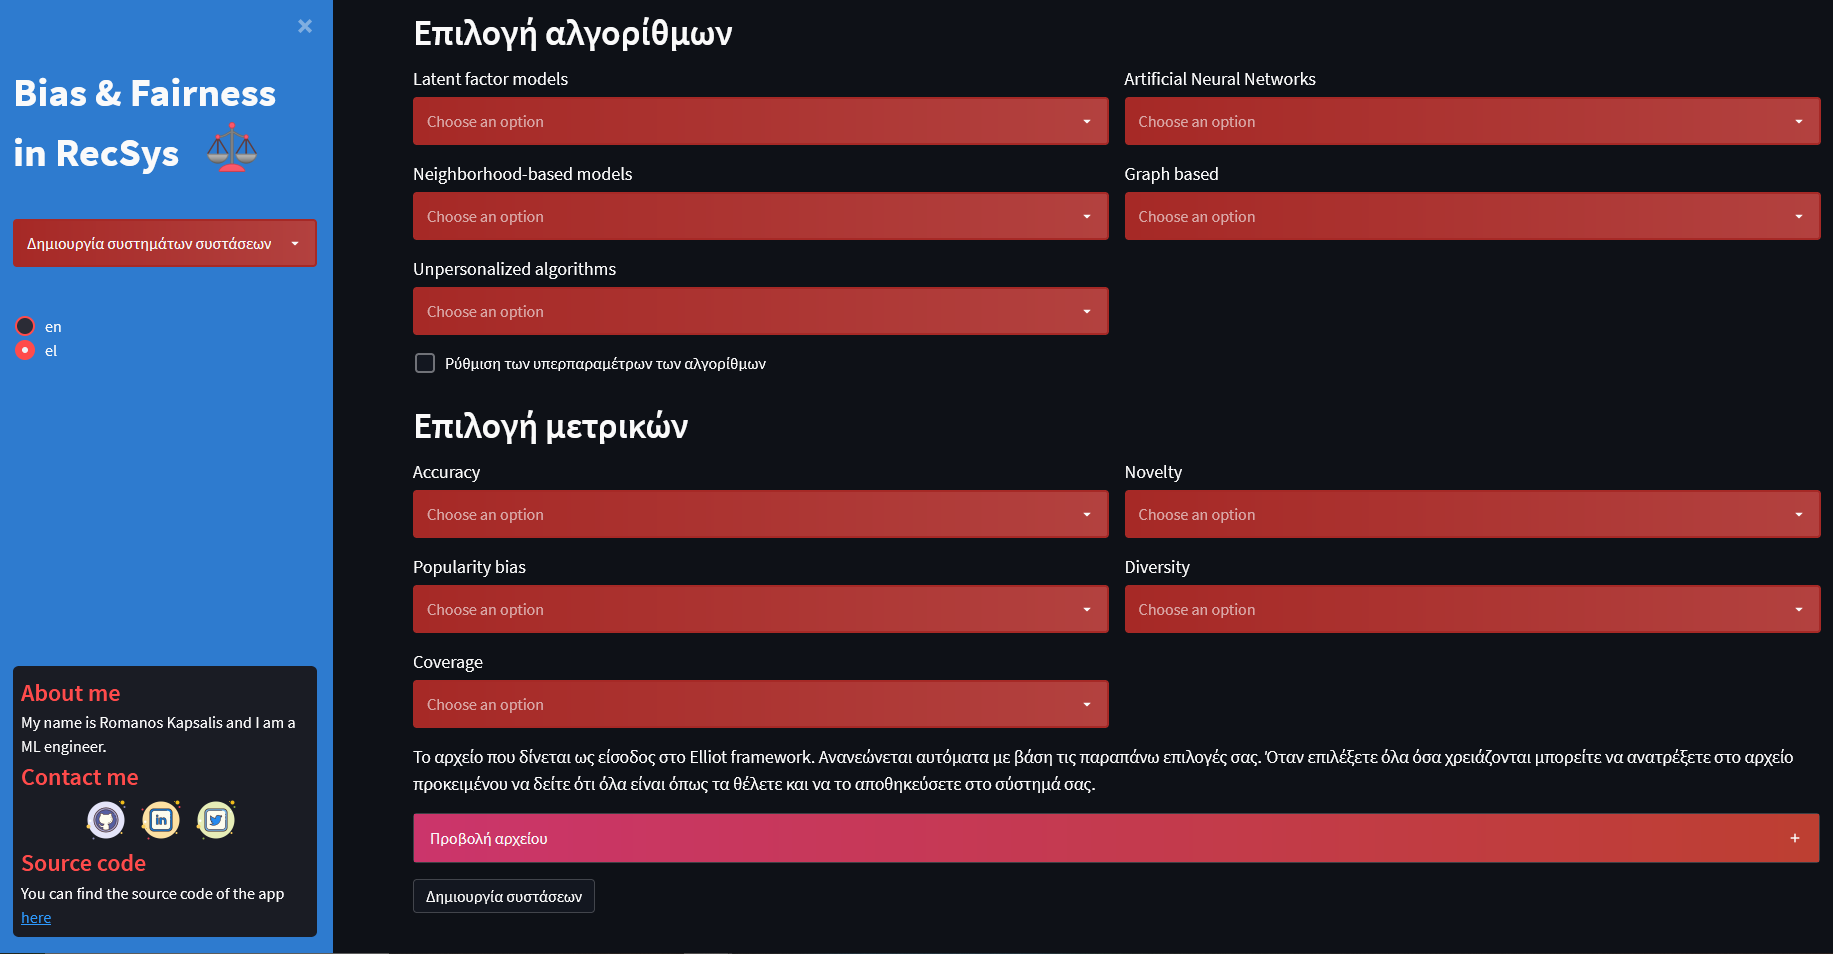
\includegraphics[width=\linewidth]{build_recs_el_1.png}
	\caption{Σελίδα δημιουργίας συστήματος συστάσεων}
	\label{fig:build2}
\end{figure}
Ακριβώς κάτω από το σημείο της σελίδας στο οποίο γίνεται η επιλογή των αλγορίθμων, υπάρχει το checkbox «Ρύθμιση των υπερπαραμέτρων των αλγορίθμων», το οποίο εάν πατηθεί μας επιτρέπει να ρυθμίσουμε τις παραμέτρους των αλγορίθμων (hyperparameter optimization). Πιο αναλυτικά, σε αυτή την περίπτωση δεν χρησιμοποιούνται οι προκαθορισμένες παράμετροι των αλγορίθμων, αλλά ρυθμίζονται από τον ίδιο τον χρήστη. Έτσι για κάθε αλγόριθμο που έχει επιλεχθεί, δημιουργείται ένα πλαίσιο το οποίο περιέχει τις διαθέσιμες παραμέτρους για αυτόν. Εντός αυτού του πλαισίου υπάρχουν επίσης δύο κουμπιά «Προσθήκη» και «Διαγραφή». Η ρύθμιση των παραμέτρων είναι διαθέσιμη για όλες τις οικογένειες αλγορίθμων εκτός από την unpersonalized, καθώς για τους αλγορίθμους που ανήκουν σε αυτή την οικογένεια δεν υπάρχουν παράμετροι για να ρυθμιστούν. Επειδή ωστόσο αυτή η επιλογή απαιτεί καλή γνώση των αλγορίθμων και δυνητικά μπορεί να αυξήσει σημαντικά το υπολογιστικό κόστος, κρίθηκε αναγκαίο να υπάρχει κατάλληλη προειδοποίηση. Στην Εικόνα \ref{fig:build3} δίνεται ένα παράδειγμα ρύθμισης των παραμέτρων των αλγορίθμων BPRMF και NGCF.\\
\begin{figure}[!htb]
	%\vspace{2px}%
	\centering
	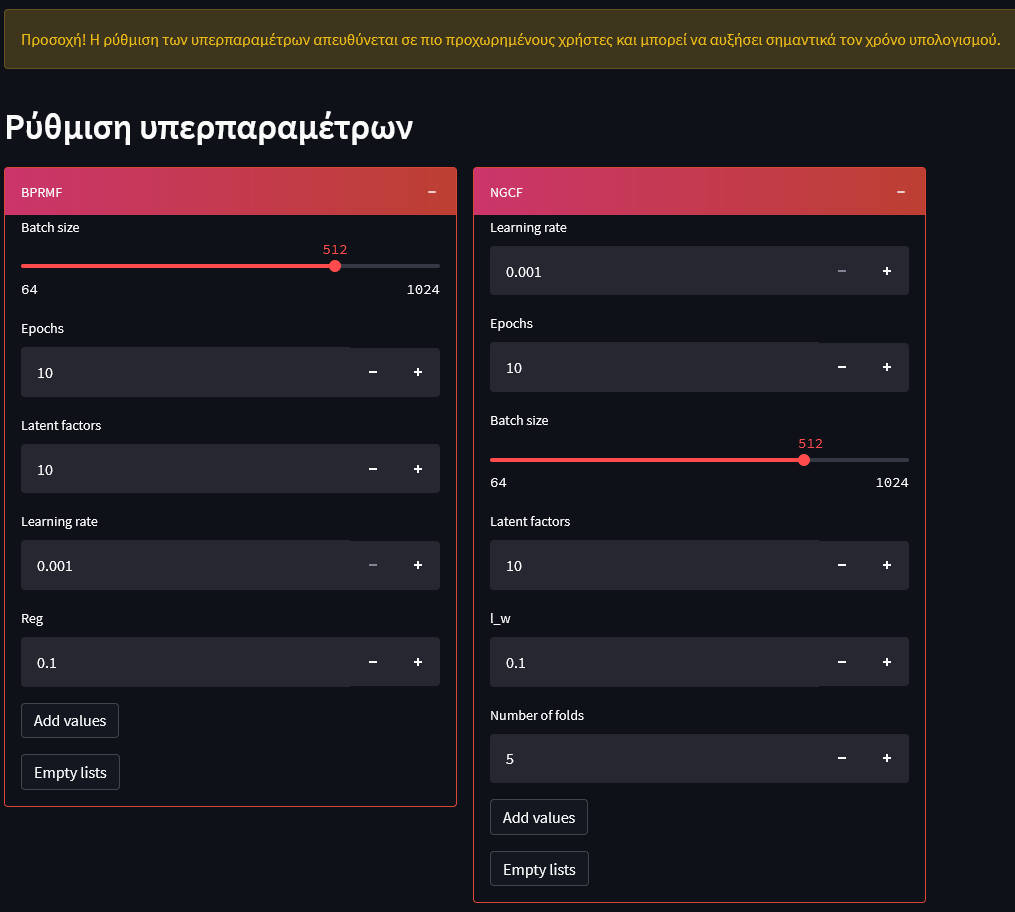
\includegraphics[width=\linewidth]{hyper_tuning.png}
	\caption{Ρύθμιση υπερπαραμέτρων των αλγορίθμων BPRMF και NGCF μέσω της εφαρμογής}
	\label{fig:build3}
\end{figure}
Ένα ακόμη απαραίτητο στοιχείο για την διεξαγωγή ενός πειράματος είναι φυσικά οι μετρικές αξιολόγησης, και αυτές, όπως και οι αλγόριθμοι, είναι κατηγοριοποιημένες. Οι κατηγορίες είναι: ακρίβεια, popularity bias, diversity, novelty και coverage.
Προκειμένου να διευκολύνουμε όσο περισσότερο γίνεται όλους τους χρήστες, υπάρχει η δυνατότητα προβολής του αρχείου yml που χρησιμοποιεί το Elliot, το οποίο δημιουργείται αυτόματα από την εφαρμογή μας και ανανεώνεται δυναμικά καθώς ο χρήστης εισάγει ή διαγράφει μια μετρική ή έναν αλγόριθμο και τις παραμέτρους. Μάλιστα, αφού ολοκληρωθεί η επιλογή όλων των στοιχείων του πειράματος και βεβαιωθεί ο χρήστης πως δεν έχει κάνει κάποιο λάθος, παρέχεται η δυνατότητα να κατεβάσει το συγκεκριμένο αρχείο στη συσκευή του, πατώντας το κουμπί «Λήψη αρχείου».\\ Τέλος, μετά τη ρύθμιση όλων των παραπάνω στοιχείων, πατώντας το κουμπί «Δημιουργία», ξεκινάει η δημιουργία των λιστών συστάσεων από τους αλγορίθμους που έχουν επιλεγεί και η αξιολόγηση των αποτελεσμάτων από τις μετρικές αξιολόγησης, μέσω του Elliot.
Τα αρχεία αποτελεσμάτων που έχουν δημιουργηθεί αποθηκεύονται προσωρινά στο σύστημα έως ότου ο χρήστης να κλείσει την εφαρμογή.\\
Από όλα τα παραπάνω συνάγεται το συμπέρασμα ότι το σύστημα που αναπτύξαμε, δεν αποτελεί μόνο ένα εργαλείο για τον εντοπισμό και τον μετριασμό της μεροληψίας αλλά και ένα εργαλείο για τη δημιουργία συστημάτων συστάσεων με αρκετά φιλικό τρόπο προς τους χρήστες
\newpage
\section{Αξιολόγηση αποτελεσμάτων}
\noindent Σε αυτή τη σελίδα γίνεται η ανάλυση των αποτελεσμάτων, δηλαδή των λιστών συστάσεων για κάθε χρήστη, που έχουν παράξει οι αλγόριθμοι του Elliot. Η ανάλυση μπορεί να γίνει είτε επιλέγοντας τα αποτελέσματα που αφορούν ένα σύνολο δεδομένων είτε μπορεί να γίνει σύγκριση διαφορετικών συνόλων δεδομένων.\\\\
\textbf{1. Επιλογή ενός συνόλου δεδομένων}\\
Εάν επιλεγεί να γίνει η ανάλυση των αποτελεσμάτων ενός μόνο συνόλου δεδομένων, τότε αρχικά θα πρέπει να επιλέξουμε τον τύπο ή τους τύπους της ανάλυσης που επιθυμούμε. Υπάρχουν διαθέσιμοι τρεις τύποι ανάλυσης των αποτελεσμάτων: προβολή καλύτερων αποτελεσμάτων, ανάλυση υπερπαραμέτρων και ανάλυση cut-off, με  τον προεπιλεγμένο τύπο ανάλυσης να είναι η προβολή των καλύτερων αποτελεσμάτων.
\\Στη συνέχεια, γίνεται η επιλογή ενός συνόλου δεδομένων. Για όλα τα σύνολα δεδομένων η εύρεση και η ανάγνωση των αρχείων αποτελεσμάτων γίνεται αυτόματα από το σύστημα χωρίς να απαιτείται καμία περαιτέρω ενέργεια του χρήστη. Ωστόσο, όπως γίνεται αντιληπτό για το σύνολο δεδομένων που έχει μεταφορτώσει ο χρήστης, απαραίτητη προϋπόθεση είναι να έχει δημιουργήσει πρώτα συστήματα συστάσεων μέσω της σχετικής σελίδας της εφαρμογής. 

\noindent Επόμενο βήμα αποτελεί η επιλογή των μετρικών αξιολόγησης. Οι μετρικές αξιολόγησης είναι κατηγοριοποιημένες, ακριβώς όπως και στη σελίδα «Δημιουργία συστημάτων συστάσεων». Έπειτα, ανάλογα με τον τύπο ανάλυσης των αποτελεσμάτων προβάλλονται τα σχετικά γραφήματα. \\ \\
\textbf{Προβολή καλύτερων αποτελεσμάτων}\\
Στην προβολή των καλύτερων αποτελεσμάτων προβάλλονται τα καλύτερα αποτελέσματα που έχουν προκύψει σε κάθε διαθέσιμη τιμή cut-off, δηλαδή ο καλύτερος συνδυασμός των τιμών όλων των υπερπαραμέτρων και ο χρήστης έχει τη δυνατότητα να επιλέξει την τιμή του cut-off που επιθυμεί.\\
\begin{figure}[!htb]
	%\vspace{2px}%
	\centering
	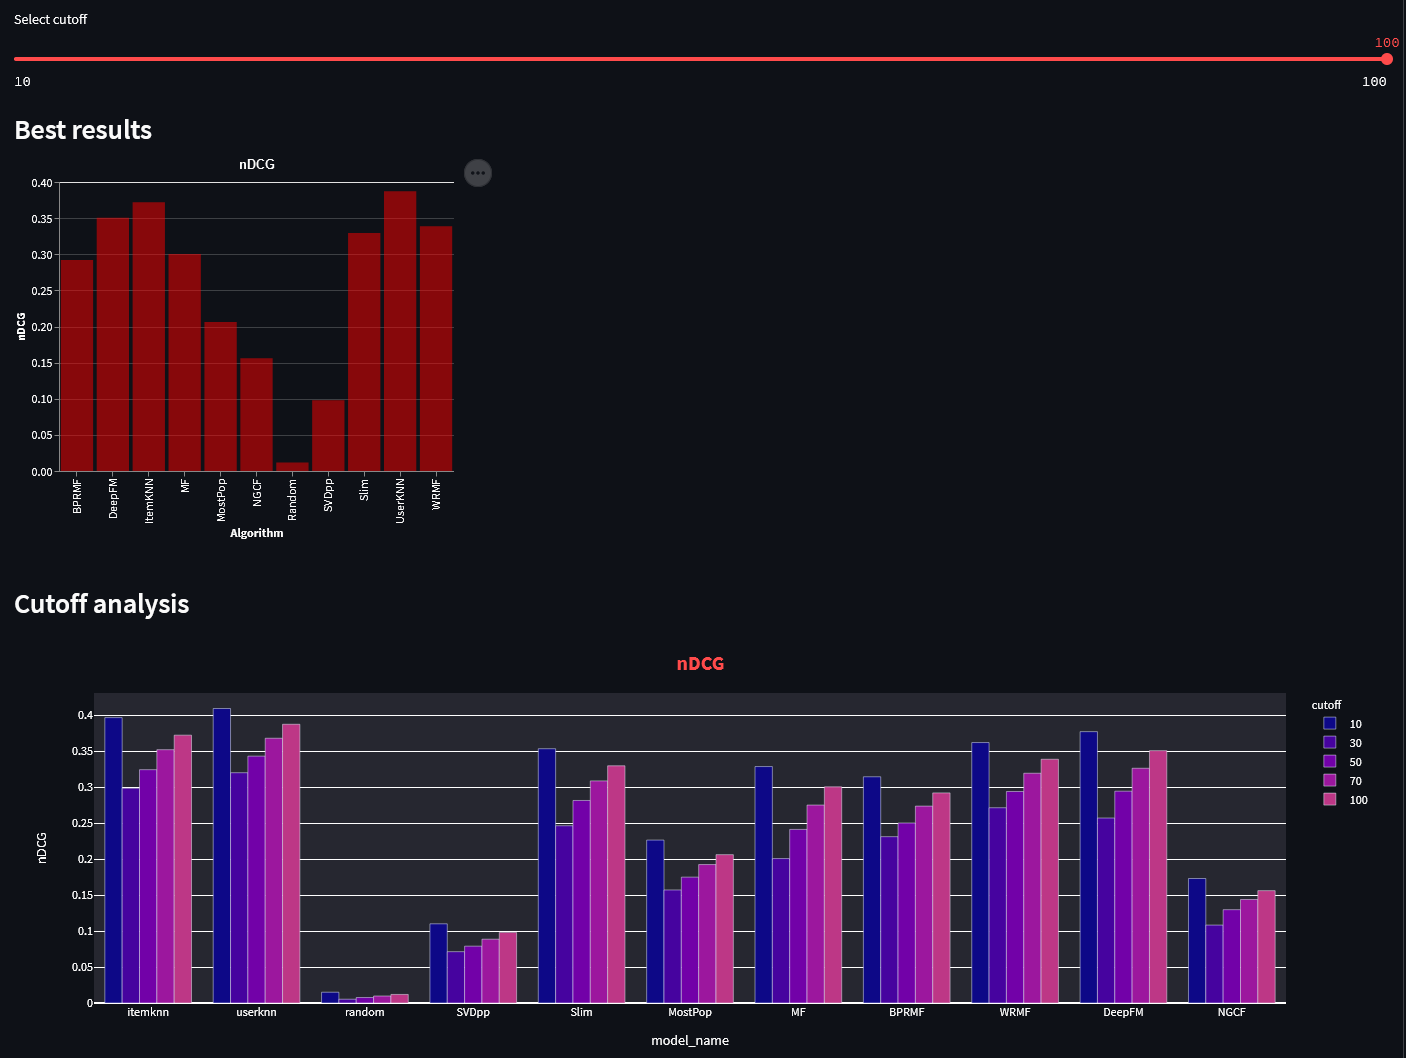
\includegraphics[width=\linewidth]{Screenshot 2021-11-05 225158.png}
	\caption{Παράδειγμα προβολής καλύτερων αποτελεσμάτων και ανάλυσης cut-off}
	\label{fig:best}
\end{figure}
\\
\textbf{Ανάλυση cut-off}\\
Η διαφορά της ανάλυσης cut-off από την προβολή των καλύτερων αποτελεσμάτων είναι στο είδος των γραφημάτων που παρουσιάζονται και πως δεν χρειάζεται να επιλεγεί κάποια τιμή cut-off. Πιο συγκεκριμένα, προβάλλονται οι τιμές που έχουν προκύψει για όλες τις τιμές cut-off σε ένα γράφημα για όλους τους αλγορίθμους και για μια επιλεγμένη μετρική.\\\\
\newpage
\noindent \textbf{Ανάλυση υπερπαραμέτρων}
\\ Αυτός ο τύπος ανάλυσης χρειάζεται εκτός από το σύνολο δεδομένων και τις μετρικές αξιολόγησης, και την επιλογή του αλγορίθμου ή των αλγορίθμων, του οποίου ή των οποίων οι παράμετροι θα αναλυθούν. Αφού επιλεγεί ο αλγόριθμος, τότε ο χρήστης επιλέγει επίσης και τις παραμέτρους που θέλει και με τη σειρά που θέλει. Η μια παράμετρος είναι εκείνη που θα βρίσκεται στον άξονα x και η άλλη καθορίζει το πλήθος των γραμμών (με άλλα λόγια καθορίζει ποια υπερπαράμετρος θα χρησιμοποιηθεί για να κωδικοποιηθούν οι μοναδικές τιμές της μέσω διαφορετικών χρωμάτων). Εάν ο αριθμός των παραμέτρων ενός αλγορίθμου είναι μεγαλύτερος του 3, τότε υπάρχει και μια τρίτη παράμετρος που μπορεί να επιλεγεί και αφορά την μεταβλητή που θα κρατηθεί σταθερή. Δηλαδή, θα δημιουργηθούν τόσα γραφήματα, όσες και οι τιμές της παραμέτρου. Εάν επιλεγεί να γίνει σύγκριση διαφορετικών συνόλων δεδομένων, υπάρχει διαθέσιμος μόνο ένας τύπος ανάλυσης, η προβολή των καλύτερων αποτελεσμάτων. Αυτό συμβαίνει διότι η ανάλυση των υπερπαραμέτρων για έναν αλγόριθμο σε διαφορετικά σύνολα δεδομένων, είναι μια αρκετά σύνθετη και δύσκολη διαδικασία, καθώς τα σύνολα δεδομένων πολλές φορές διαφέρουν κατά πολύ μεταξύ τους, με κυριότερη διαφορά το πολύ μεγάλο εύρος τιμών cut-off που μπορούμε να συναντήσουμε. Επομένως, θα πρέπει να ληφθούν υπόψη αρκετές παράμετροι, κάτι που δεν εξετάστηκε στην παρούσα εργασία και αποτελεί αντικείμενο μελλοντικής εργασίας.
\newpage
\begin{figure}[H]
	%\vspace{2px}%
	\centering
	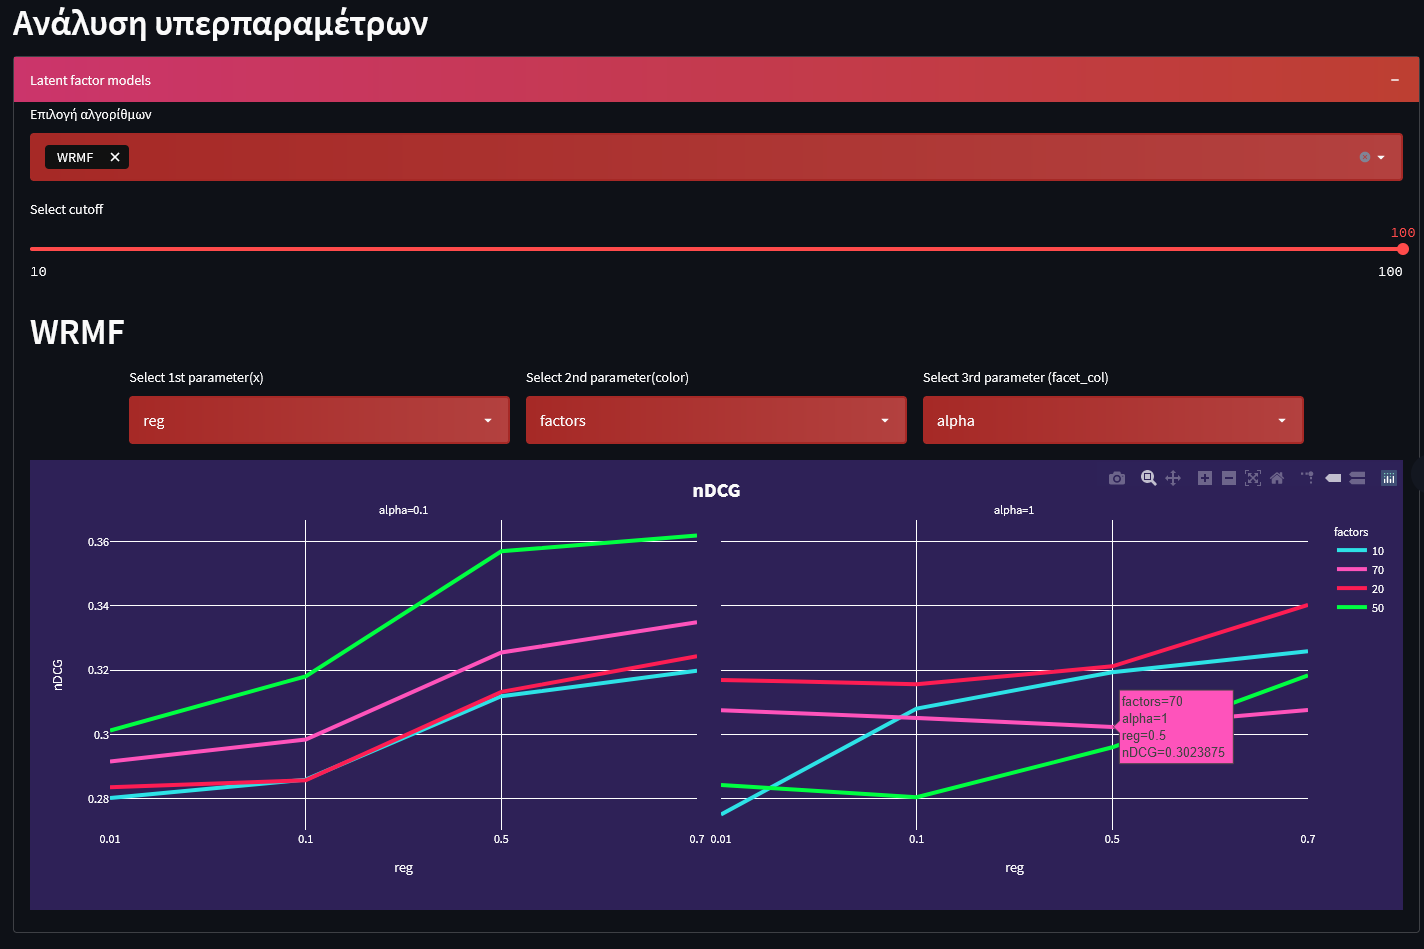
\includegraphics[width=\linewidth]{analyze_hyper.png}
	\caption{Παράδειγμα ανάλυσης υπερπαραμέτρων.}
	\label{fig:hyper}
\end{figure}
\noindent \textbf{2. Σύγκριση διαφορετικών συνόλων δεδομένων}
\\Στη σύγκριση διαφορετικών συνόλων δεδομένων (Εικόνα \ref{fig:hyper}) ο χρήστης μπορεί να συγκρίνει τα αποτελέσματα όπως αυτά προέκυψαν από διαφορετικά σύνολα δεδομένων και έχει δύο επιλογές. Η πρώτη είναι να καθορίσει ο ίδιος τα σύνολα δεδομένων που επιθυμεί, εάν προηγουμένως έχει μεταφορτώσει τα αρχεία που εμπεριέχουν τα καλύτερα αποτελέσματα για κάθε cut-off για όλους τους αλγορίθμους, για κάποιο σύνολο δεδομένων που έχει στην κατοχή του ο χρήστης (περισσότερες λεπτομέρειες θα βρείτε στην υποενότητα «Μεταφόρτωση δεδομένων»). Ενώ η δεύτερη είναι η σύγκριση όλων των προτύπων συνόλων δεδομένων. Σε αυτή την έκδοση της εφαρμογής είναι διαθέσιμη μόνο η 2η επιλογή, οι λόγοι που οδήγησαν σε αυτόν τον περιορισμό περιγράφονται αναλυτικά στην ενότητα \ref{limitations} του Κεφαλαίου 6. Και στις δύο περιπτώσεις, όπως και στην «Επιλογή ενός μόνο συνόλου δεδομένων», εμφανίζονται γραφήματα για κάθε μετρική που έχει προεπιλεγεί.
\newpage
\begin{figure}[H]
	%\vspace{2px}%
	\centering
	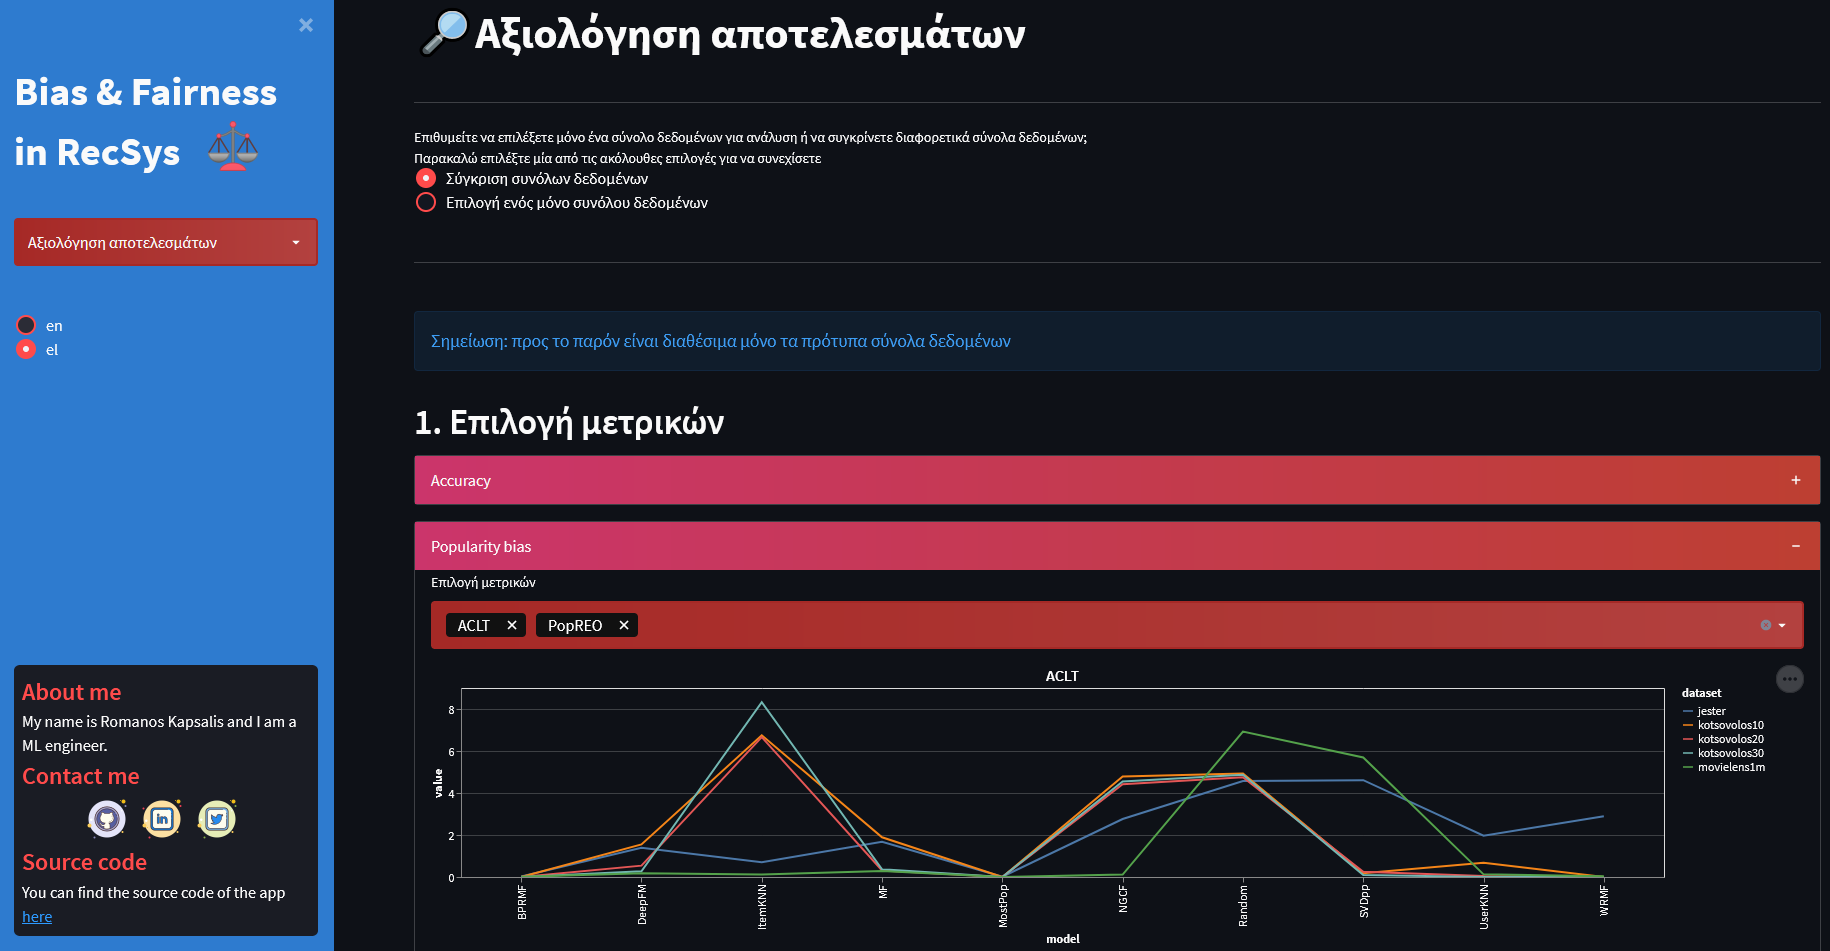
\includegraphics[width=\linewidth]{bias_ident.png}
	\caption{Παράδειγμα σύγκρισης συνόλων δεδομένων.}
	\label{fig:compare}
\end{figure}
%%%%%%%%%%%%%%%%%%%%%%%%%%%%%%%%%%%%%%%%%%%%%%%%%%%%%
%%             ΜΕΤΡΙΑΣΜΟΣ ΜΕΡΟΛΗΨΙΑΣ               %%
%%%%%%%%%%%%%%%%%%%%%%%%%%%%%%%%%%%%%%%%%%%%%%%%%%%%%
\section{Μετριασμός μεροληψίας}
\begin{figure}[H]
	%\vspace{2px}%
	\centering
	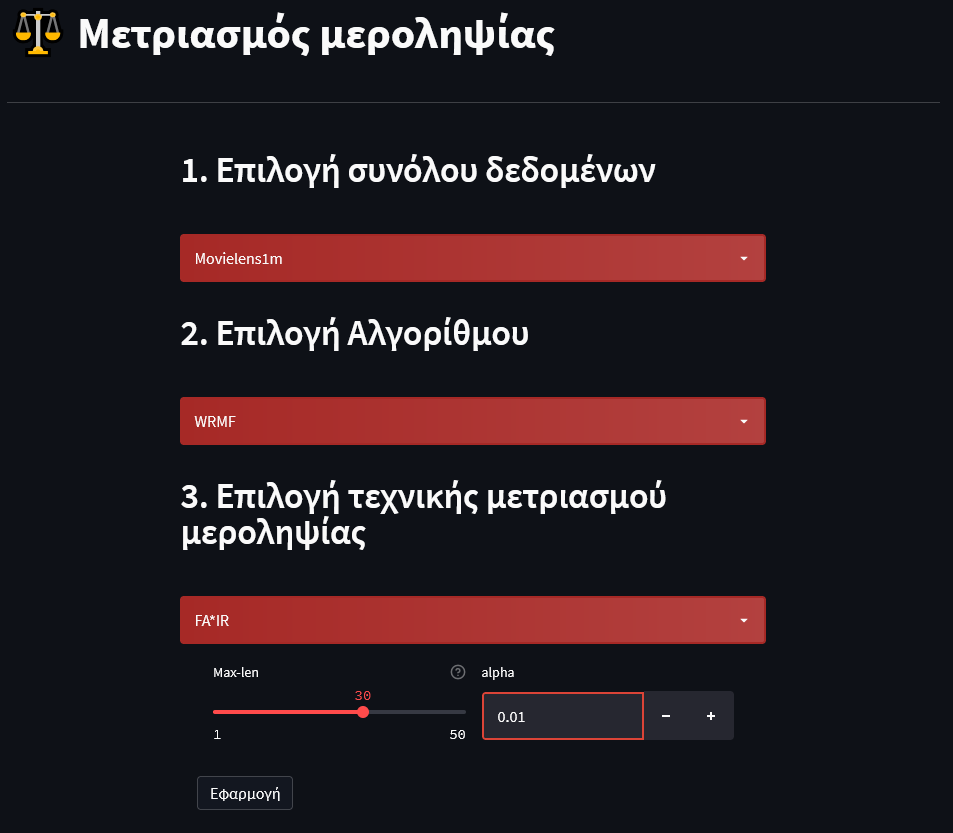
\includegraphics[width=\linewidth]{bias_mitigation.png}
	\caption{Σελίδα μετριασμού μεροληψίας}
	\label{fig:mitigation}
\end{figure}
\noindent Η σελίδα αυτή υλοποιεί το βήμα του πειράματος κατά το οποίο γίνεται ο μετριασμός του popularity bias που έχει εντοπιστεί σε ένα σύστημα συστάσεων. Όταν ο χρήστης επισκέπτεται αυτή τη σελίδα, τότε μπορεί είτε να διαβάσει αναλυτικές πληροφορίες για τους αλγορίθμους μετριασμού της μεροληψίας και για τη διαδικασία γενικότερα, είτε να μετριάσει κατευθείαν την μεροληψία σε έναν αλγόριθμο, εάν είναι εξοικειωμένος με τη διαδικασία.\\ Ο μετριασμός της μεροληψίας αποτελείται από τρία αρκετά απλά βήματα. Αρχικά, και όπως σε όλα τα βήματα που έχουμε περιγράψει έως τώρα, γίνεται η επιλογή του συνόλου δεδομένων και έπειτα η επιλογή του αλγορίθμου ο οποίος δημιούργησε τις λίστες συστάσεων στις οποίες πιθανώς εντοπίσαμε την ύπαρξη μεροληψίας μέσω της σελίδας «Ανάλυση δεδομένων». Προφανώς η λίστα με τους διαθέσιμους αλγόριθμους αλλάζει και ανανεώνεται δυναμικά, κάθε φορά που επιλέγουμε κάποιο σύνολο δεδομένων. Μετά την επιλογή του αλγορίθμου, σειρά έχει η επιλογή της τεχνικής που επιθυμούμε να εφαρμόσουμε για τον μετριασμό της μεροληψίας. Υπάρχουν τέσσερις διαθέσιμες τεχνικές οι οποίες ανήκουν όλες στην κατηγορία των post-processing αλγορίθμων, και πιο συγκεκριμένα τεχνικές που αναδιατάσσουν (re-ranking) μια λίστα συστάσεων. Οι αλγόριθμοι αυτοί είναι οι FAR, PFAR, FA*IR και Calibrated Recommendations (Cali) τους οποίους έχουμε περιγράψει εκτενώς στην Ενότητα 3 και προέρχονται από το framework Librec-auto. Σε αυτούς δίνονται ως είσοδος η λίστα συστάσεων για κάθε χρήστη που έχει δημιουργήσει ο base αλγόριθμος, καθώς και ένα αρχείο τύπου csv, που περιέχει όλα τα IDs των αντικειμένων και τον χαρακτηρισμό long ή head, αν ανήκει στο long tail και στο head, αντίστοιχα για καθένα από αυτά. Ένα παράδειγμα τέτοιου αρχείου δίνεται στην Εικόνα \ref{fig:feature}. Για τον αλγόριθμο FA*IR υπάρχει προειδοποίηση προς τους χρήστες ότι ανάλογα με το μέγεθος του συνόλου δεδομένων ο υπολογισμός του μπορεί να είναι εξαιρετικά αργός.
\begin{figure}[H]
	%\vspace{2px}%
	\centering
	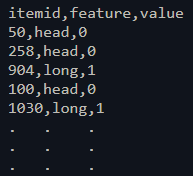
\includegraphics[]{item_features.png}
	\caption{Παράδειγμα αρχείου item features στο Movielens100k}
	\label{fig:feature}
\end{figure}
 \noindent Αξίζει να σημειωθεί ότι για την εύρεση του αρχείου που έδωσε τα καλύτερα αποτελέσματα γίνεται πρώτα η ανάγνωση ενός αρχείου τύπου json που έχει δημιουργήσει το Elliot και περιέχει τις καλύτερες παραμέτρους. Κάθε ένας από αυτούς τους αλγορίθμους περιέχει και δύο παραμέτρους τις οποίες θα πρέπει να ρυθμίσει ο χρήστης. Η μία παράμετρος είναι το μέγεθος των λιστών συστάσεων για κάθε χρήστη, αυτό θα πρέπει σε κάθε περίπτωση να είναι μικρότερο από το αρχικό μέγεθος, και η άλλη παράμετρος καθορίζει τον βαθμό ισορροπίας ανάμεσα στην ακρίβεια και στη μεροληψία. Για την εφαρμογή της επιλεγμένης τεχνικής μετριασμού της μεροληψίας αρκεί το πάτημα του κουμπιού «Εφαρμογή». Αφού ολοκληρωθεί η διαδικασία, τότε γίνεται η αξιολόγηση των νέων λιστών που έχουν παραχθεί, χρησιμοποιώντας τις μετρικές αξιολόγησης που είχαν χρησιμοποιηθεί και στο πείραμα κατά το οποίο δημιουργήθηκαν οι αρχικές λίστες συστάσεων. Ο χρήστης ενημερώνεται με σχετικά μηνύματα που προβάλλονται στην οθόνη για την πρόοδο τόσο του μετριασμού της μεροληψίας, όσο και της αξιολόγησης των αποτελεσμάτων. Τέλος, και με προϋπόθεση την επιτυχή έκβαση των δύο παραπάνω διαδικασιών, στον χρήστη παρουσιάζονται τα αποτελέσματα των μετρικών αξιολόγησης μέσω γραφημάτων.
\newpage
\section{Επεξήγηση μετρικών}
\noindent Αναφερθήκαμε προηγουμένως στην αναγκαιότητα αυτή η εφαρμογή να μπορεί να χρησιμοποιηθεί και από άτομα χωρίς ιδιαίτερες τεχνικές γνώσεις. Σε αυτό το πλαίσιο, δημιουργήθηκε μια ακόμη σελίδα η οποία περιγράφει κάθε μετρική που είναι διαθέσιμη στο Elliot, σε γλώσσα απλή και κατανοητή για όλους τους χρήστες ανεξαρτήτως των γνώσεων τους. Για παράδειγμα, στην Εικόνα \ref{fig:explain} ο χρήστης έχει επιλέξει να προβάλλει την επεξήγηση για την μετρική ACLT. Προς διευκόλυνση του χρήστη υπάρχει η δυνατότητα ανάπτυξης όλων των πλαισίων, μέσω απλής επιλογής στο πάνω δεξιό μέρος της οθόνης («Ανάπτυξη όλων»), ενώ οι μετρικές είναι κατηγοριοποιημένες σε 5 κατηγορίες.
\begin{figure}[H]
	%\vspace{2px}%
	\centering
	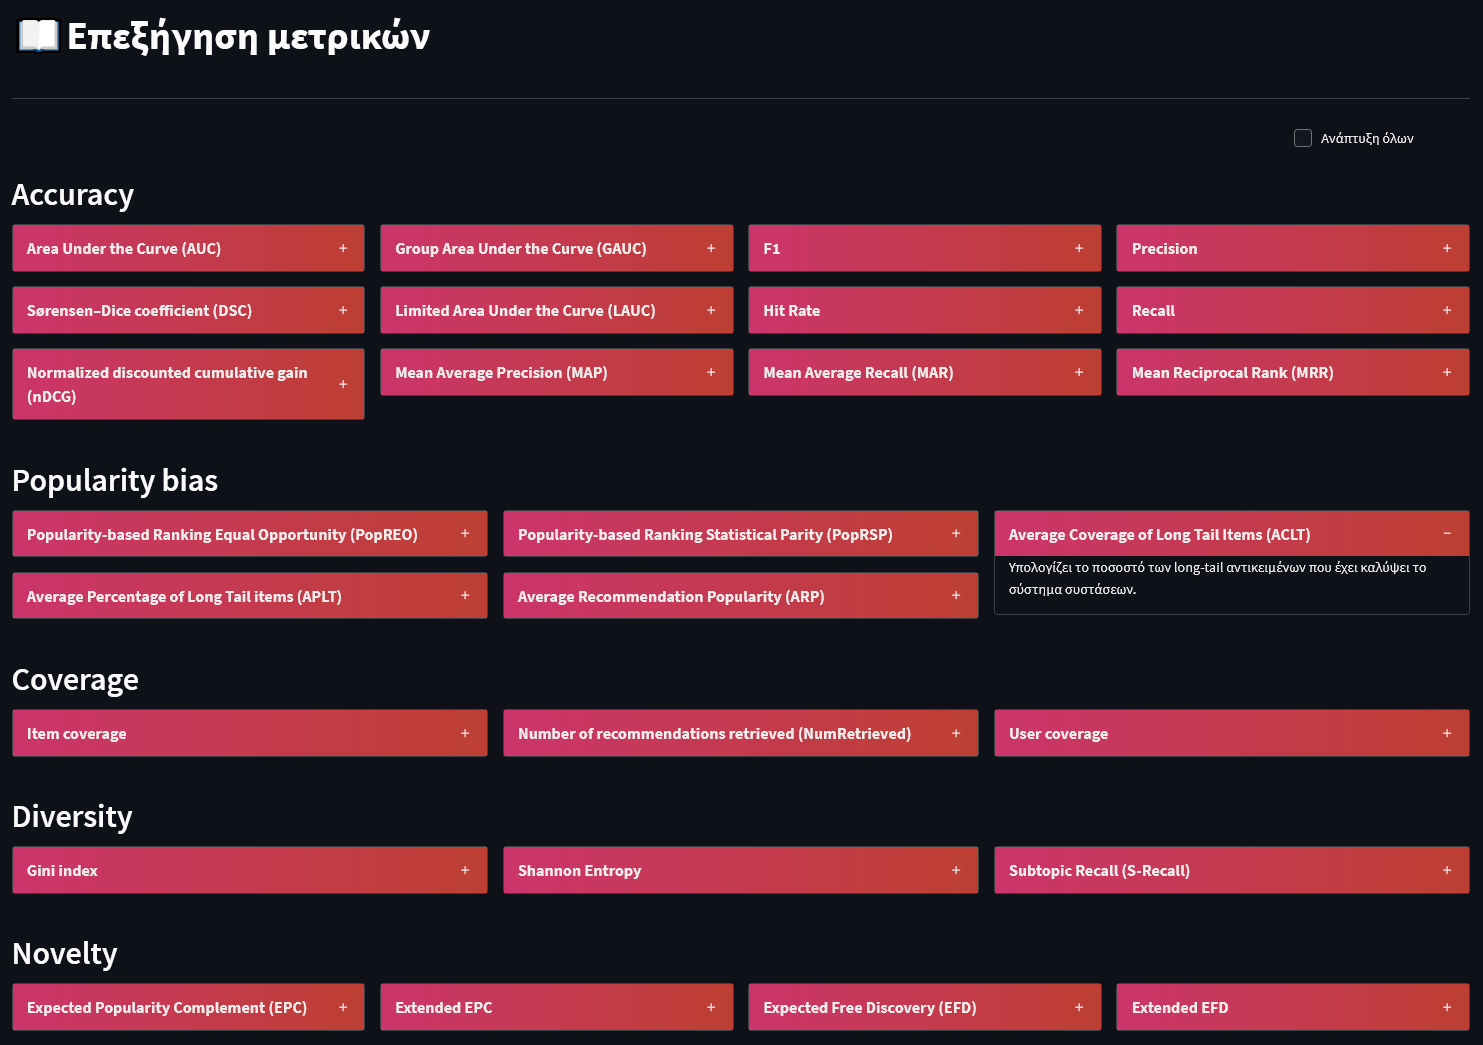
\includegraphics[width=\linewidth]{explanations4.png}
	\caption{Σελίδα επεξήγησης μετρικών αξιολόγησης.}
	\label{fig:explain}
\end{figure}
\noindent Οι επεξηγήσεις των μετρικών συμβάλλουν στην επεξηγησιμότητα, στοχεύοντας σε μια μελλοντική επέκταση της εφαρμογής και προς αυτήν την κατεύθυνση.
\newpage
\section{Μεταφόρτωση δεδομένων}
\noindent Εκτός από τα πρότυπα σύνολα δεδομένων τα οποία χρησιμοποιήθηκαν στο πείραμά μας και είναι διαθέσιμα για επιλογή και χρήση στην εφαρμογή, ο χρήστης μπορεί να μεταφορτώσει το δικό του σύνολο δεδομένων. Το σύνολο δεδομένων αποθηκεύεται τοπικά στην μνήμη RAM και παραμένει σε αυτή έως ότου ο χρήστης κλείσει την εφαρμογή με οποιονδήποτε τρόπο ή ανανεώσει την ιστοσελίδα της εφαρμογής. Με αυτόν τον τρόπο, διασφαλίζουμε στους χρήστες πως δεν έχουμε πρόσβαση στα δεδομένα τους, καθώς αυτά δεν αποθηκεύονται κάπου.\\
%\clearpage
\begin{figure}[H]
	%\vspace{2px}%
	\centering
	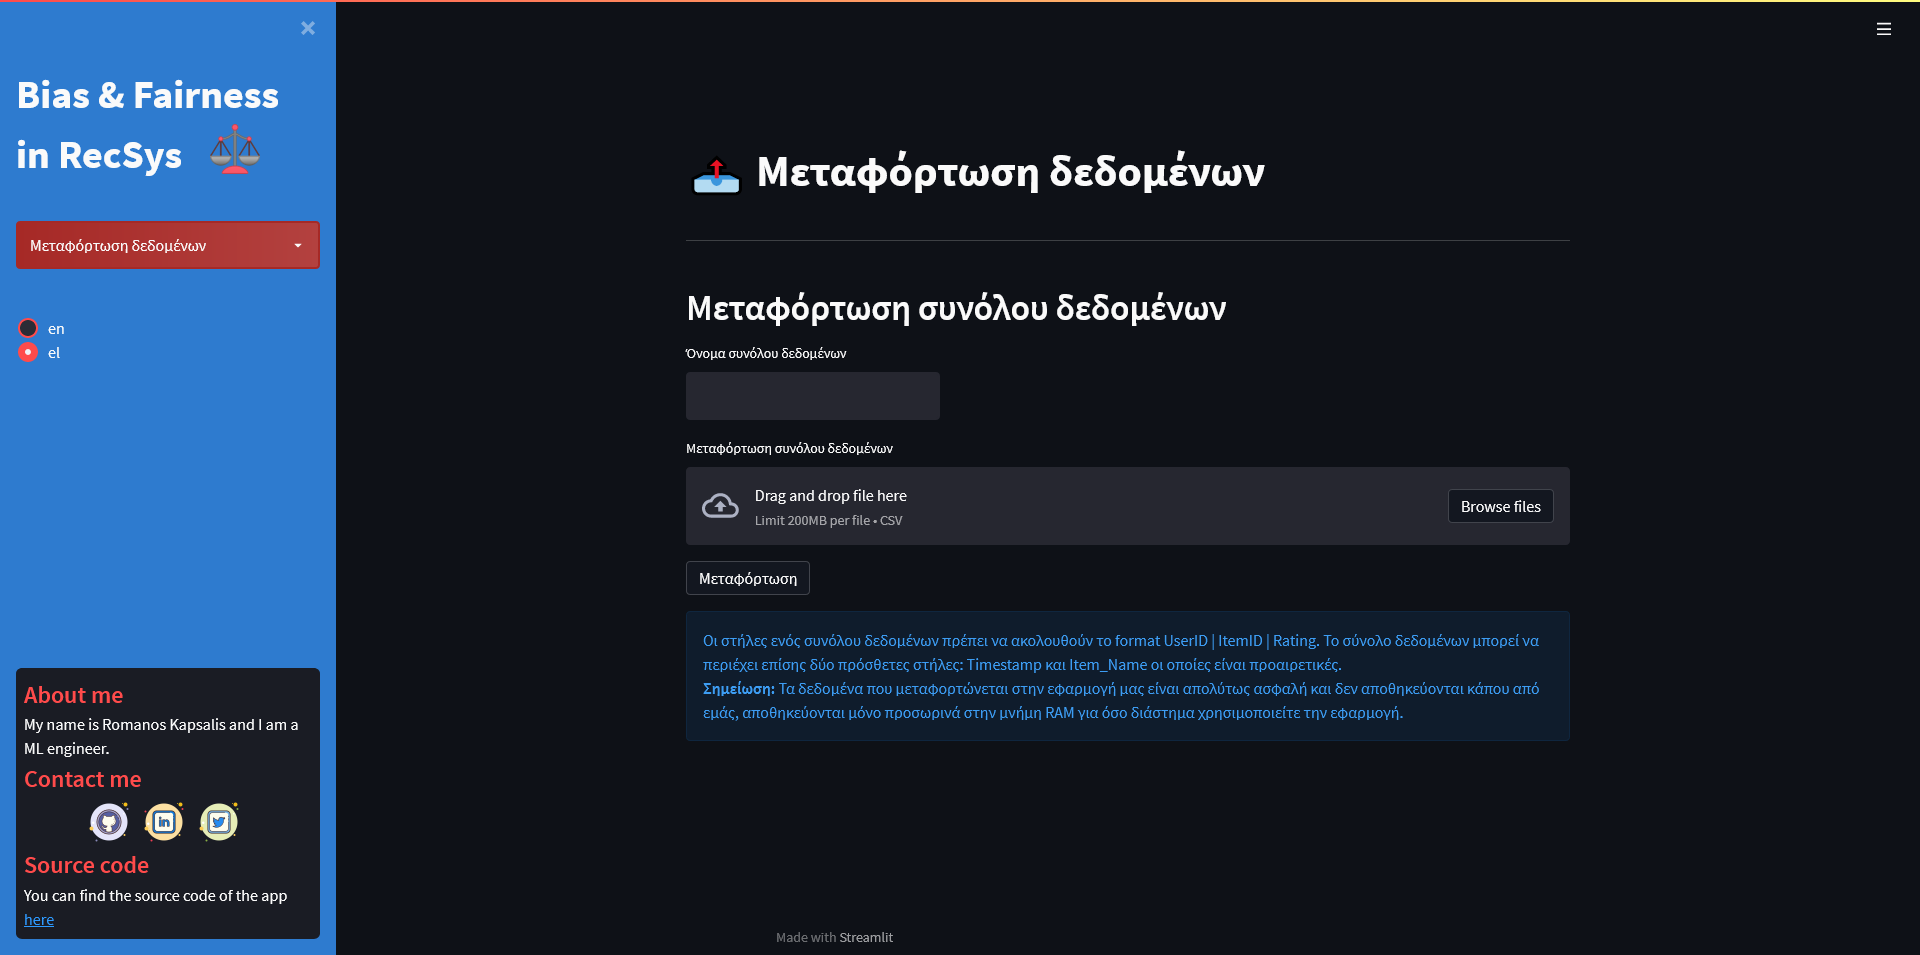
\includegraphics[width=\linewidth]{upload.png}
	\caption{Σελίδα μεταφόρτωσης δεδομένων.}
	\label{fig:upload}
\end{figure}
\noindent Η εφαρμογή υποστηρίζει δύο τύπους αρχείων ``.tsv" και ``.csv", ενώ θα πρέπει να επισημάνουμε πως το μέγιστο μέγεθος του συνόλου δεδομένων που θα μεταφορτωθεί δεν θα πρέπει να ξεπερνάει τα 200mb, για λόγους που σχετίζονται με την ομαλή λειτουργία και απόδοση του συστήματος. Πιο συγκεκριμένα, μετριάζουμε τον κίνδυνο να υπερχειλίσει η μνήμη RAM, προκαλώντας πολυάριθμα προβλήματα. Ένας ακόμη περιορισμός που έχουμε εισάγει είναι πως το σύνολο δεδομένων θα πρέπει να περιέχει υποχρεωτικά τρεις στήλες: User ID, Item ID και Rating, ενώ προαιρετικά μπορεί να περιέχει και δύο επιπλέον στήλες, τη στήλη ``Timestamp", η οποία θα περιέχει την ακριβή χρονική στιγμή που υποβλήθηκε μια αξιολόγηση για ένα προϊόν από κάποιον χρήστη και τη στήλη ``Item\_Name", η οποία θα περιέχει το όνομα κάθε αντικειμένου.


